\documentclass[uplatex]{jsarticle}
\usepackage[dvipdfmx]{graphicx}
\usepackage{ascmac}
\usepackage{listings}
\usepackage{amsmath}
\usepackage{bm}
\usepackage{cases}

\DeclareMathOperator*{\minimize}{minimize}


\title{人工知能 課題番号1「人工知能の実現可能性について考察せよ」}
\author{工学部電子情報工学科 03-175001 浅井明里}

\makeatletter
\def\maketitle{%
  \null
  \thispagestyle{empty}%
  \vfill
  \begin{center}\leavevmode
    \normalfont
    {\LARGE \@title\par}%
    \vskip 1cm
    {\Large \@author\par}%
    \vskip 1cm
    {\Large \@date\par}%
  \end{center}%
  \vfill
  \null
  \@thanks%\vfil\null
  \cleardoublepage
  }
\makeatother


\title{人工知能 課題番号17「ゲームのモンテカルロ木(UCT)探索を用いたゲームの探索プログラム」}
\author{工学部電子情報工学科 03-175001 浅井明里}
\date{\today}

\begin{document}
\maketitle

% \section{モンテカルロ探索法とは}
% \subsection{モンテカルロ探索法と従来の手法との相違点}

\section{3次元 Tit-for-tatにおけるモンテカルロ探索法とminimax探索法の対戦}
本課題では4 x 4 x 4という三次元におけるTic-for-tatゲームでモンテカルロ探索法とminimax探索法を対戦させ、
探索の効率(展開されたノードの数)及び勝敗数を元に比較を行なった。プログラムについては授業及び講義サイトで紹介されている、
3次元Tit-for-tat(4x4x4)のプログラム(その2)の評価関数を拡張するなどの実装を行なった。

\subsection{minmax法の評価関数の改善}
今回は以下の二つの評価手法によりある手を売った場合の盤面の評価値を算出し、$\alpha\beta$を導入した
minimax法により最善手を求めた。
\begin{itemize}
  \item 評価関数1 : 盤面のそれぞれのマスを重み付けし、その時点で自身が取得しているマスのスコアの合計を評価値とする。
  \item 評価関数2 : 現時点の盤面から自身が勝利する、実現可能なpathの数から相手にとって実現可能な勝利path数をひき、定数倍したものを評価値とする。
  \item 評価関数3 : 盤面のそれぞれの行、列に対して、いくつ自身で埋められているかに応じてスコアを与え、合計を評価値とする。
\end{itemize}

\subsubsection{評価関数1}
この評価関数ではそれぞれの局面の盤面のそれぞれのセルを順に見ていき、そのセルが敵の駒で埋められていればそのセルにつけられたスコアを$-1$
倍したものを、自分の駒で埋められていればそのセルに割り当てられたスコアを足していき、その合計値を最終的な評価値とする。

評価関数はminimax.cのget\_evaluation\_value()という関数で定義されている。
\subsubsection{評価関数2}
この評価関数では「あといくつ勝利するためのパスが残されているか」を数え上げ、その合計に100をかけて評価値とする。
具体的にどう「勝利可能なパス」を求め、また評価値を算出するかを図1に示す。
\begin{figure}
  \begin{center}
    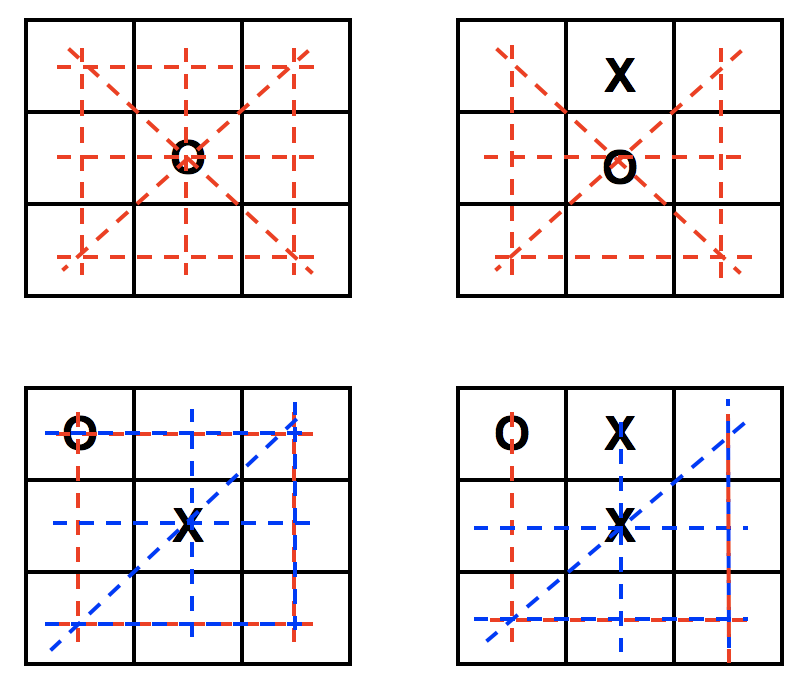
\includegraphics[width=13cm]{img/eval_2.png}
    \caption{勝利Pathの計算}
  \end{center}
\end{figure}
例えば「O」の勝利するために実現可能なpathを考える。図1左上の盤面では、中央に「O」があるのみであるため、
まだ全ての行、列及び対角線のpathのいずれかで「O」が埋め、勝利をする可能性がある。
よって図1左上の盤面での「O」にとって勝利可能なパスの数は8通り、同様にして、右上の盤面では「O」のすぐ上を
「X」が埋めてしまっているため、勝利可能なパスの数は6通りに減少している。
評価値はこれと同様の計算を相手側についても行い、
$$評価値 = ((自分の勝利可能なパスの数) - (相手の勝利可能なパスの数)) \times C,\ Cは自然数 $$
で算出する。
例えば図1の右下の盤面では、「O」は4通りの勝利パスが、「X」は6通りの勝利パスが存在するため、
この盤面の評価値は
$$(4 - 6) \times 100 = -200$$となる。

評価関数はminimax.cのget\_evaluation\_value\_heuristics()という関数で定義されており、
この関数の内部でヘルパー関数として、いくつまだ実現可能なパスが残されているか計算する
get\_possible\_win(koma\_type mycolor, const koma\_type board[HEIGHT][AREA])
を呼ぶ。この関数ではあるパスについて相手が駒を置いていないかチェックし、まだ相手側が駒を置いていなければ
勝利可能パスとして登録する。

\begin{lstlisting}[basicstyle=\ttfamily\footnotesize, frame=single]
// 4. Check the vertical among different hights. MAX = AREA(16)
for (j = 0; j < AREA; j++) {
  int tmp = 0;
  for (i = 0; i < HEIGHT; i++) {
    tmp = (board[i][j] != REVERSE(mycolor)) ? tmp + 1 : tmp;
  }
  if (tmp == 4) {
    possible_wins += 1;
  }
}
\end{lstlisting}

三次元Tic Tac Towでは、ある一つの状態につき複数の盤面が存在するため、それぞれの盤面に登場する
勝利パスを足し合わせ、最後に相手側の勝利パス数の合計をひいいた上で定数項をかける。



\subsubsection{評価関数3}
この評価関数では、それぞれの局面の盤面の行、列の埋まり具合から「全て埋めることができた」「自身がすでに3つ埋めていて、残り一つのセルが空白である」
「自身が2つ埋めている」「相手が3つ埋めていて残り一つが空白である」「相手が全て埋めた」などのケースそれぞれに一定のスコアを付与し、
その合計を評価値とする。スコアは以下のように、どちらかが全ての列もしくは行を埋めた場合の評価値をより絶対値を大きくなるように
設定している。

\begin{lstlisting}[basicstyle=\ttfamily\footnotesize, frame=single]
  int convert_cell_num_to_score(int enemy_cell_num, int my_cell_num,
                                int empty_cell_num) {
    if (my_cell_num == 4) {
      return 2000;
    } else if (my_cell_num == 3) {
      return 600 + 50 * empty_cell_num;
    } else if (my_cell_num == 2) {
      return 100 - 100 * enemy_cell_num + 50 * empty_cell_num;
    } else if (my_cell_num == 1) {
      return -600 + empty_cell_num * 50;
    } else {
      return -2000;
    }
  }
\end{lstlisting}

評価関数はminimax.cのget\_evaluation\_value\_dynamic()という関数で定義されている。

\section{結果の分析}
\subsection{探索効率の比較}
探索効率については、UTC法とそれぞれの評価関数を用いたminimax法を対戦させ、
一つの手を求めるためにかかった時間を計測した。図2, 3, 4, 5はそれぞれ
UTC法、評価関数2を用いたMiniMax法($\alpha \beta 枝刈るを行なったもの$),
評価関数3を用いたMiniMax法($\alpha \beta 枝刈るを行なったもの$),
評価関数4を用いたMiniMax法($\alpha \beta 枝刈るを行なったもの$)
のそれぞれの手を求めるためにかかった時間をゲームごとに平均したものをプロットしている。
UTC方についてはステップアウト数の増加とともに計算時間が増加する傾向があるが、MiniMax法では
必ずしもこの傾向が観測できるわけではない。また評価関数3については他の二つの評価関数より
計算時間が長くなっている傾向にある。これは評価関数3が他の二つの関数より評価値のばらつきが小さく、
枝刈りの効率が悪いからではないかと推測する。また、UTC法はMiniMax法の手法よりも計算時間が短く済んでおり、
効率的に探索できていると言える。

\begin{figure}[htbp]
\begin{minipage}{0.5\hsize}
 \begin{center}
  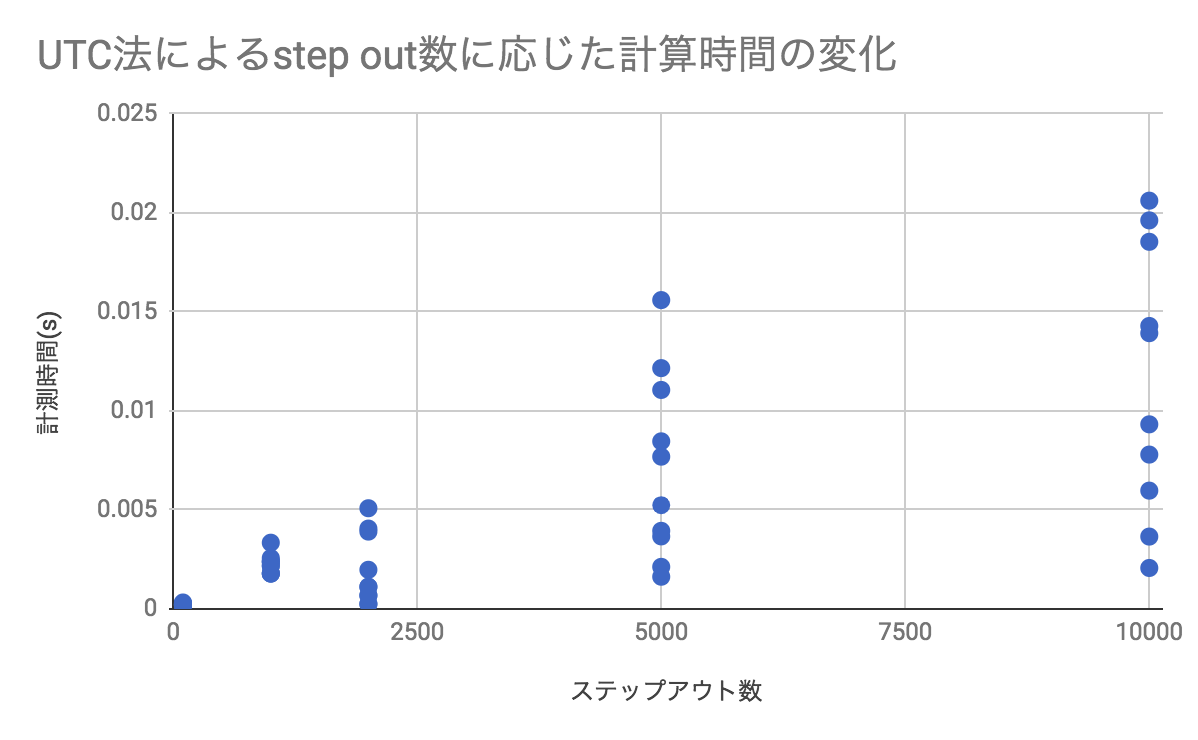
\includegraphics[width=80mm]{img/calc_time_1.png}
 \end{center}
 \caption{UTC法での計算時間}
 \label{fig:one}
\end{minipage}
\begin{minipage}{0.5\hsize}
 \begin{center}
  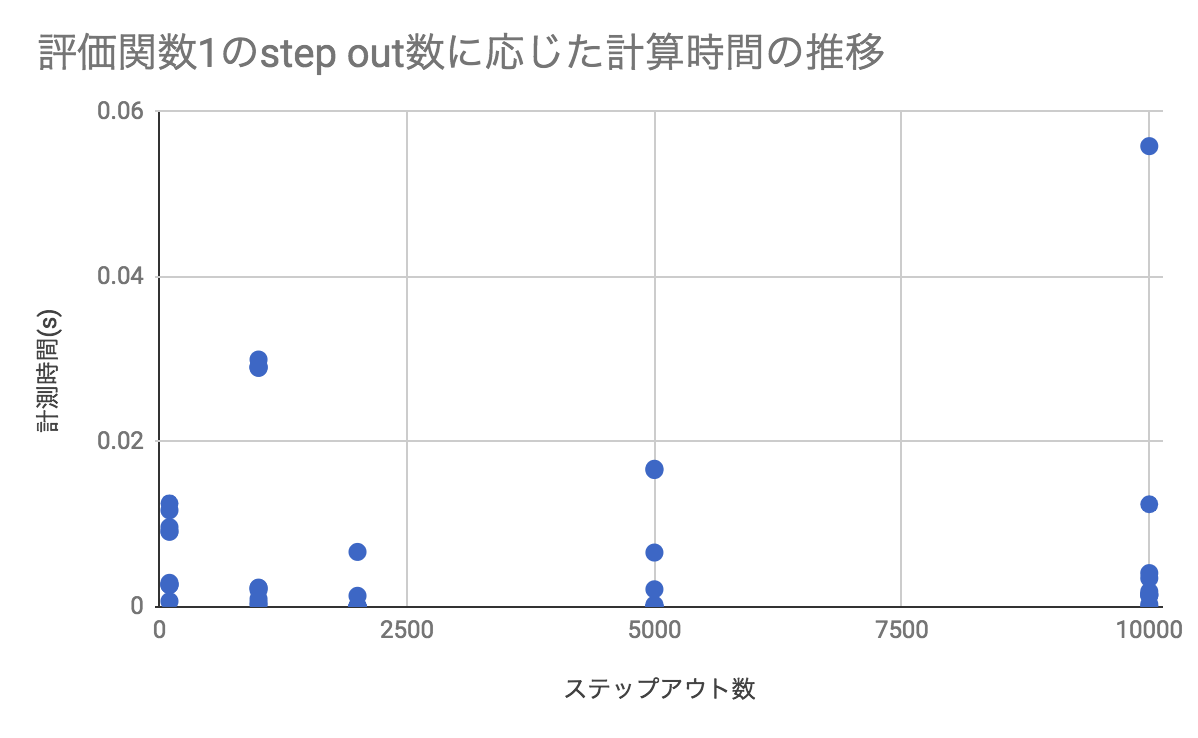
\includegraphics[width=80mm]{img/calc_time_2.png}
 \end{center}
 \caption{評価関数1を用いたMiniMax法での計算時間}
 \label{fig:two}
\end{minipage}
\end{figure}

\begin{figure}[htbp]
\begin{minipage}{0.5\hsize}
 \begin{center}
  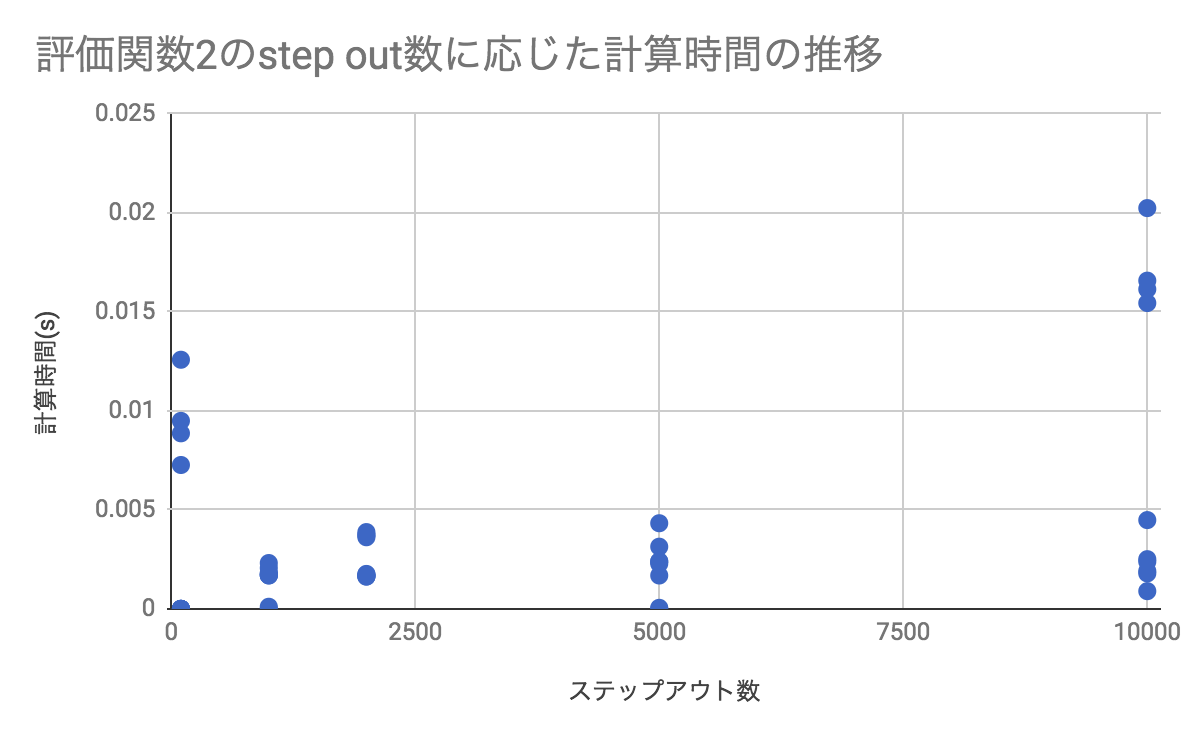
\includegraphics[width=80mm]{img/calc_time_3.png}
 \end{center}
 \caption{評価関数2を用いたMiniMax法での計算時間}
 \label{fig:one}
\end{minipage}
\begin{minipage}{0.5\hsize}
 \begin{center}
  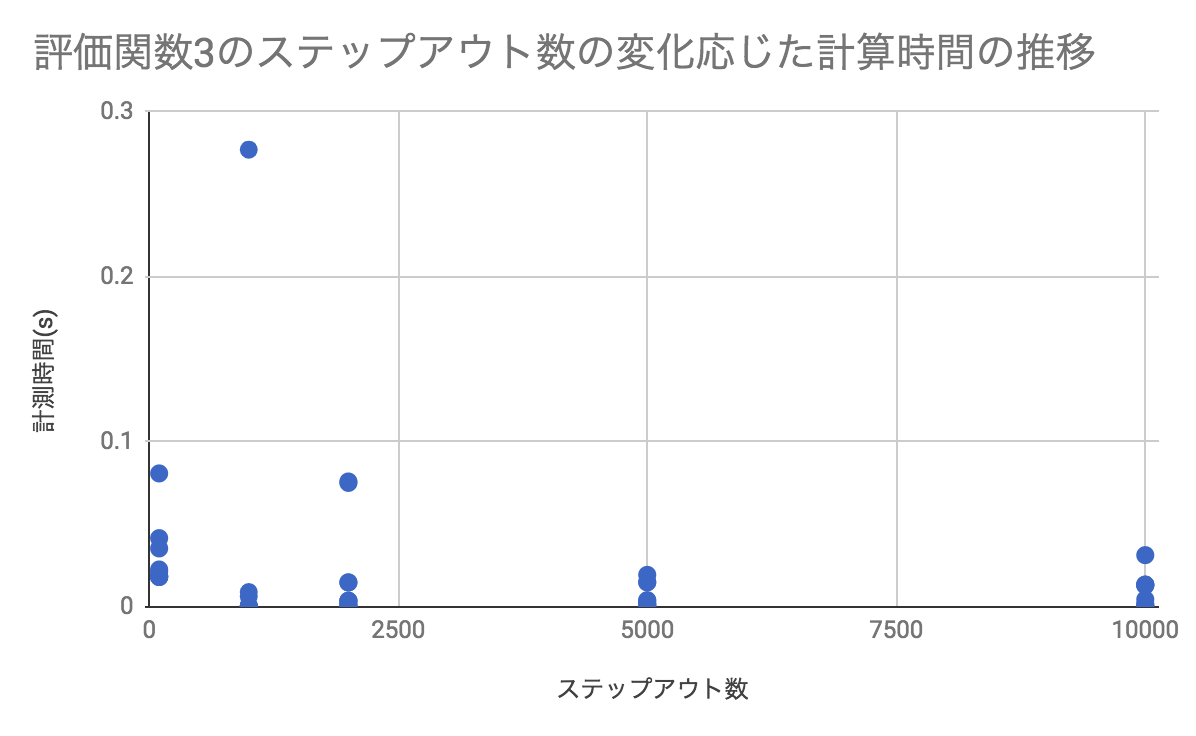
\includegraphics[width=80mm]{img/calc_time_4.png}
 \end{center}
 \caption{評価関数3を用いたMiniMax法での計算時間}
 \label{fig:two}
\end{minipage}
\end{figure}

\subsection{勝率の推移}
図6に示した二つの表は、評価関数をそれぞれ変えたMiniMax方に対するUTC法の勝率ををステップアウト数ごとに
一覧にしたものである。表の単位は\%である。UTC法はステップアウト数が10000程度までの時には
MiniMax法に全体として劣っているが、ステップアウト数が100000ではUTC法が圧倒的な勝率を見せている。
評価関数2が先攻の際と後攻の際で勝率が大きく異なっているが、これは「勝てるパスを探す」という評価の仕方が、
先攻の法が残り勝利パスが大きくなりやすいために、有利に働くからではないかと推測する。一方で、
そもそもステップアウト数が10000の時点でのモンテカルロ法の強さは初期値に依存するために、実験時のモンテカルロ法の
プレーヤーが「良くない」初期解を引いたという可能性も否定はできない。

\begin{figure}
  \begin{center}
    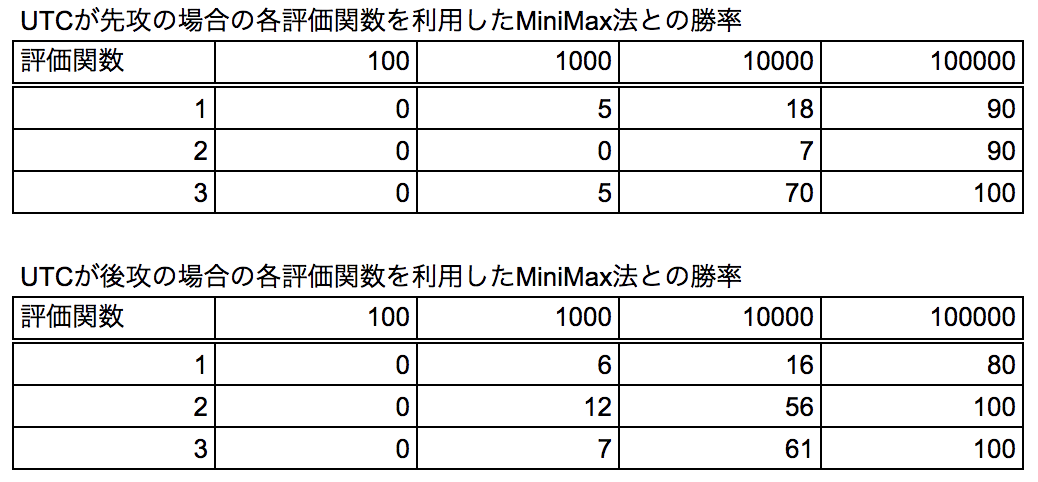
\includegraphics[width=15cm]{img/table.png}
    \caption{UTC法の勝率の変化}
  \end{center}
\end{figure}





\begin{thebibliography}{9}
  \bibitem{evans} Thomas H. Cormen, Charles E. Leiserson, Ronald L. Rivest, Clifford Stein.
    "Introduction to Algorithms", MIT Press, 2009.
  \bibitem{iba} 伊庭斉志,
    『人工知能と人工生命の基礎』, オーム社 , 2013.
\end{thebibliography}


\end{document}
